\documentclass[%margin%,line,pifont,palatino,courier
]{article}
\usepackage{fullpage}
\usepackage{lastpage}
\usepackage[top=1in,bottom=1in,margin=1in]{geometry}
\usepackage{supertabular}
\usepackage{graphicx,tikz}	
%\usepackage{tkz-euclide}
%\usetkzobj{all}
%\usetikzlibrary{calc}
\usepackage{array,multicol}
\usepackage{amsmath,amssymb}
\usepackage{enumitem}

\usepackage{fancyhdr}
\pagestyle{fancy}

\addtolength{\topmargin}{-0.25in}

\newcommand{\vect}[1]{\mathbf{#1}}
\DeclareMathOperator{\proj}{proj}

\fancypagestyle{plain}{
	\addtolength{\headheight}{0.485in}
	\rhead{\bf MATH 236 (Calculus II) \\
		%\vspace{0.5pc}
		due Wed 27 Sep 2017 \\}
	\rfoot{\footnotesize THQuiz 3, p. \thepage\ (of \pageref{LastPage})
	}
\renewcommand{\headrulewidth}{0pt}
}
\fancyhf{}
\renewcommand{\headrulewidth}{0pt}
\rfoot{\footnotesize THQuiz 3, p. \thepage\ (of \pageref{LastPage})$\;$}

\title{\vspace{-3.5pc} 
	\flushleft \bf \Large Take-Home Quiz 3: Applications of integrals %\\ 
	 (\S6.1-6.2, 6.4)}
\date{}

% % % % %
\begin{document}
\maketitle

\vspace{-3pc}
\noindent{\bf Directions:} This quiz is due on September 27, 2017 at the beginning of lecture.  You may use whatever resources you like -- e.g., other textbooks, websites, collaboration with classmates -- to complete it \textbf{but YOU MUST DOCUMENT YOUR SOURCES}.  Acceptable documentation is enough information for me to find the source myself.  Rote copying another's work is unacceptable, regardless of whether you document it.  

\noindent\hrulefill

\begin{enumerate}
% % %
\item {\bf \S6.1 \#60} Two of Dr. Geek's friends got married this year, one in June and one in July.  His traditional gift for such occasions is a fancy crystal bowl, whose volume is proportional to how much he likes the future spouse of the recipient.  The bowl given at the June wedding is pictured below, on the left.  The one given in July is pictured below, on the right. 
\vspace{-0.5pc}
\begin{center}
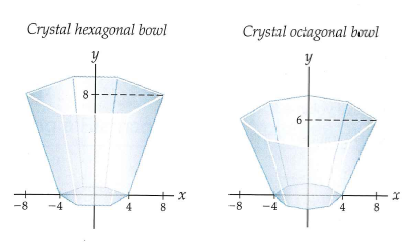
\includegraphics[scale=0.75]{6-1_60TaalmanKohn}
\end{center}
	\begin{enumerate}
	\item For the June wedding, Dr. Geek gave a fancy hexagonal crystal bowl with base hexagon of radius 4 inches, top hexagon of radius 8 inches, and height of 8 inches.  In general, the area of a hexagon with radius $r$ is $A=\frac{3\sqrt 3}{2}r^2$.  What is the volume of this bowl, in cubic inches?  \textit{(Round to one decimal.  You must explain how you got to your answer.)}
	\item For the July wedding, Dr. Geek gave a fancy octagonal crystal bowl with base radius 4, top radius 8, and height 6 inches.  In general, the area of an octagon with radius $r$ is $A=2\sqrt 2 r^2$.  What is the volume of this bowl, in cubic inches?  \textit{(Round to one decimal.  You must explain how you got to your answer.)}
	\item Whose future spouse does Dr. Geek like more?
	\end{enumerate}

% % %
\item \begin{enumerate}
	\item {\bf \S6.2 \#62} Mark carves napkin rings out of wooden spheres.  His napkin rings have height $h=8$ and radius $R=5$, measured in centimeters.  Alina also carves napkin rings out of spheres, but she likes bigger napkins, so she carves them with height $h=8$ and radius $R=6$.  Use the shell method to show that Mark's and Alina's napkin rings use exactly the same amount of wood.
\vspace{-0.5pc}
\begin{center}
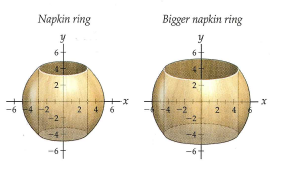
\includegraphics[scale=1]{6-2_62TaalmanKohn}
\end{center}
	\item {\bf \S6.2 \#70} Prove the \emph{Napkin Ring Theorem:} If a napkin ring is made by removing a cylinder of height $h$ from a sphere, then the volume of the resulting shape does not depend on the radius of the sphere.
	\end{enumerate}

% % %
\item {\bf \S6.4 \#60} Xander has tied a rope to a 100-pound block of ice so that he can hoist it up to his upstairs bedroom window, 22 feet off the ground.  How much work will it take for Xander to lift the block of ice up to his window, assuming that the weight of the rope is negligible but the block of ice melts off 2 pounds of water for each foot it is lifted?  \textit{You must explain how you got to your answer.}

% % %
\item {\bf \S6.4 \#66} Find the hydrostatic force exerted on a dam in the shape of an isosceles triangle whose top is 200 feet wide and whose total height is 100 feet, given that the dam is holding back a body of water that reaches to the top of the dam.  \textit{You must explain how you got to your answer.}

% % %
\item {\bf \S6.4 \#70} Ian is making snow flukes, which are metal sheets that can be used to prevent a fall on steep snow.  The flukes are in the shape of a polygon in the plane, with vertices at $(0,8)$, $(6,8)$, $(6,2)$, and $(3,\frac{1}{2})$. Lengths are in inches.

Ian needs to clip a cable to the centroid of the fluke.  Where should he attach the cable?  \textit{You must explain how you got to your answer.}

% % % % %
\end{enumerate}
\end{document}